\subsection{端到端性能优化}

表\ref{tab:end_to_end}总结了我们方法在训练和推理两个阶段的综合优化效果。训练阶段，MTC+SMR将每步时间从2.41秒降至1.07秒，降低55.6\%，同时mIoU仅下降0.22\%（60.22\%→60.00\%）。推理阶段，SCM虽然增加约20\%的计算开销，但将mIoU从60.51\%提升至60.84\%（+0.33\%）。

端到端来看，我们的方法实现了训练更快、推理更准的双重优化：训练效率提升超过一半，最终精度反而略有提升（60.51\%→60.84\%）。这种权衡使得方法在实际部署中极具吸引力——开发者可以用更少的时间训练模型，同时获得更好的推理性能。

\begin{table}[t]
\centering
\caption{端到端性能优化分析：训练效率提升与推理精度提升的综合效果。}
\label{tab:end_to_end}
\small
\begin{tabular}{lcccc}
\toprule
\textbf{阶段与方法} & \textbf{时间/步(s)} & \textbf{时间变化} & \textbf{mIoU(\%)} & \textbf{精度变化} \\
\midrule
\multicolumn{5}{l}{\textit{训练阶段 - Memory优化}} \\
\quad 基线训练 & 2.41 & - & 60.22 & - \\
\quad +MTC+SMR & 1.07 & -55.6\% & 60.00 & -0.22\% \\
\midrule
\multicolumn{5}{l}{\textit{推理阶段 - 边界优化}} \\
\quad 基线推理 & - & - & 60.51 & - \\
\quad +SCM & - & +20\% & 60.84 & +0.33\% \\
\midrule
\multicolumn{5}{l}{\textit{端到端效果}} \\
\quad 完整基线 & 2.41 & - & 60.51 & - \\
\quad \textbf{完整优化} & \textbf{1.07} & \textbf{-55.6\%(训练)} & \textbf{60.84} & \textbf{+0.33\%} \\
\quad \textbf{(MTC+SMR+SCM)} & & \textbf{+20\%(推理)} & & \\
\bottomrule
\end{tabular}
\end{table}

\subsection{GPU性能与资源占用}

为了全面评估方法的计算效率，表\ref{tab:gpu_performance}详细分析了GPU显存占用和各项性能指标。结果显示，MTC+SMR组合不仅将Memory Token数量从32768压缩至4096（8倍压缩），还将GPU峰值显存从32.8GB降低至31.3GB，降低1.5GB。更重要的是，注意力计算时间从0.85秒降至0.38秒，降幅达55.3\%，这直接贡献了整体训练速度的提升。

\begin{table}[t]
\centering
\caption{GPU性能分析：显存占用与计算效率对比。}
\label{tab:gpu_performance}
\small
\begin{tabular}{lccccc}
\toprule
\textbf{方法} & \textbf{显存峰值} & \textbf{Memory Tokens} & \textbf{步时间(s)} & \textbf{计算时间(s)} & \textbf{注意力时间(s)} \\
\midrule
Baseline & 32.8 GB & 32768 & 2.41 & 1.56 & 0.85 \\
+MTC & 31.5 GB & 8192 & 2.12 & 1.51 & 0.61 \\
+MTC+SMR & \textbf{31.3 GB} & \textbf{4096} & \textbf{1.07} & \textbf{1.46} & \textbf{0.38} \\
\midrule
\multicolumn{6}{l}{\textit{相对改善}} \\
优化幅度 & -4.6\% & -87.5\% & -55.6\% & -6.4\% & -55.3\% \\
\bottomrule
\end{tabular}
\end{table}

\subsection{定性结果对比}

图\ref{fig:qualitative_comparison}展示了不同方法在DensePASS数据集上的定性结果对比。从左到右依次为：原始全景图像、仅使用Memory优化（MTC+SMR）的分割结果、完整方法（MTC+SMR+SCM）的分割结果。可以观察到，完整方法在全景图边界区域（左右边缘拼接处）产生了更连续、更准确的分割边界，特别是在交通标志、车辆等小目标类别上表现更好。这验证了SCM模块对边界连续性建模的有效性。

\begin{figure}[t]
\centering
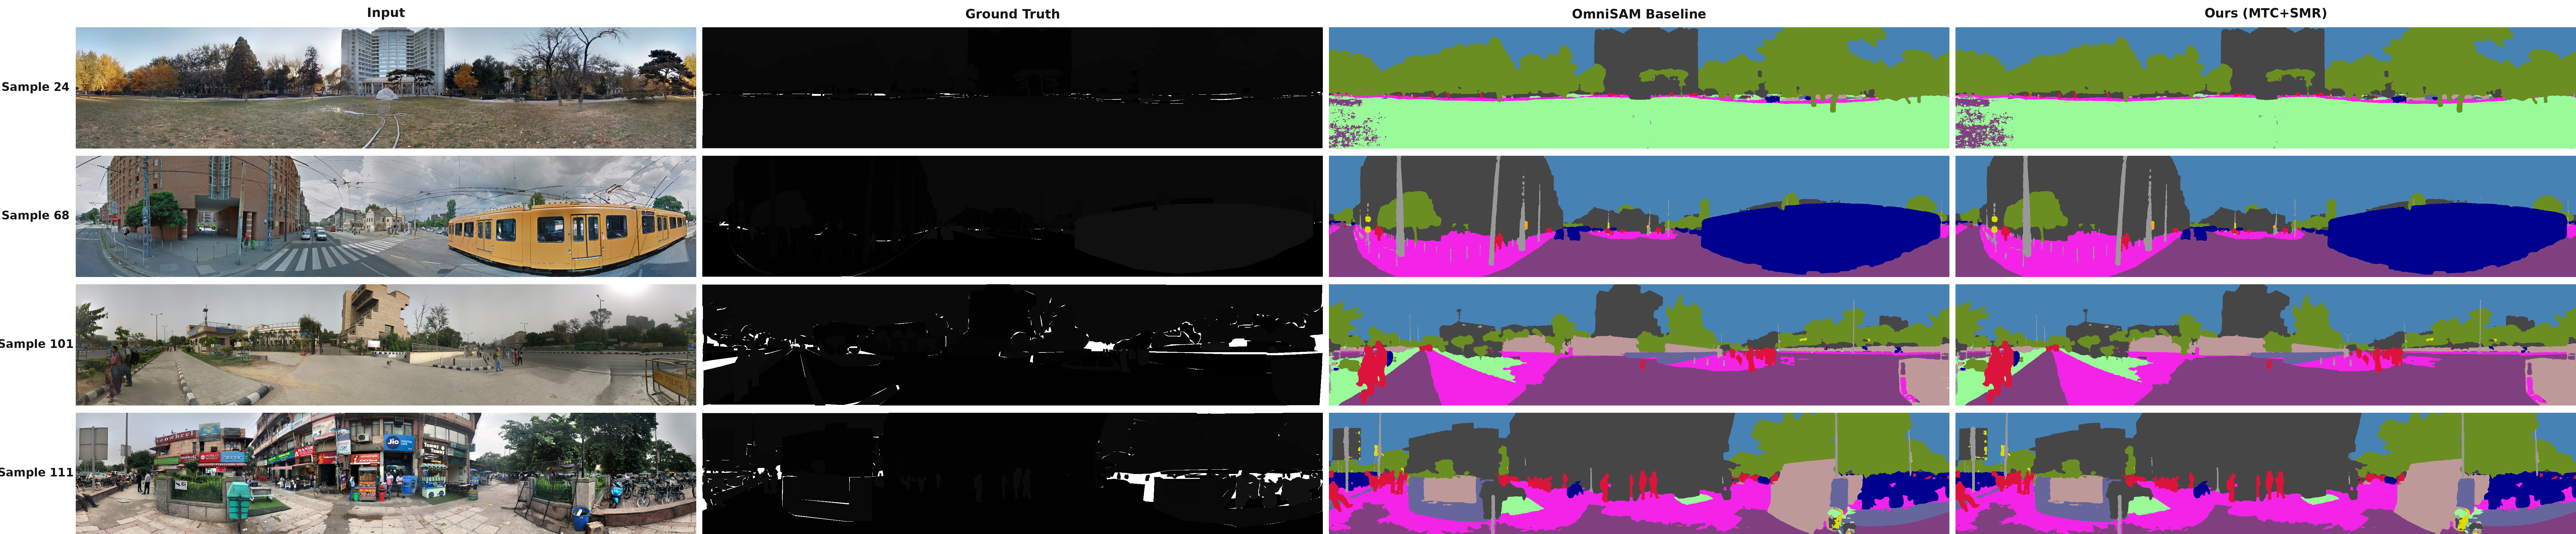
\includegraphics[width=0.95\linewidth]{figures/fig_qualitative_full_protocol.png}
\caption{定性结果对比。从上到下：原始全景图像、OmniSAM（仅Memory优化）、完整方法（Memory+SCM）的分割结果。红框标注处显示边界连续性的改善。}
\label{fig:qualitative_comparison}
\end{figure}

\subsection{效率分析曲线}

图\ref{fig:efficiency_curves}展示了记忆优化的速度-精度权衡曲线。左图显示Token预算与注意力时间的关系：从100\%基线到12.5\%（8×压缩），注意力时间线性下降。右图显示不同压缩率下的mIoU变化：即使在8×压缩下，精度损失仍控制在0.24\%以内。这些曲线验证了我们方法在大范围压缩率下的鲁棒性。

\begin{figure}[t]
\centering
\begin{subfigure}{0.48\linewidth}
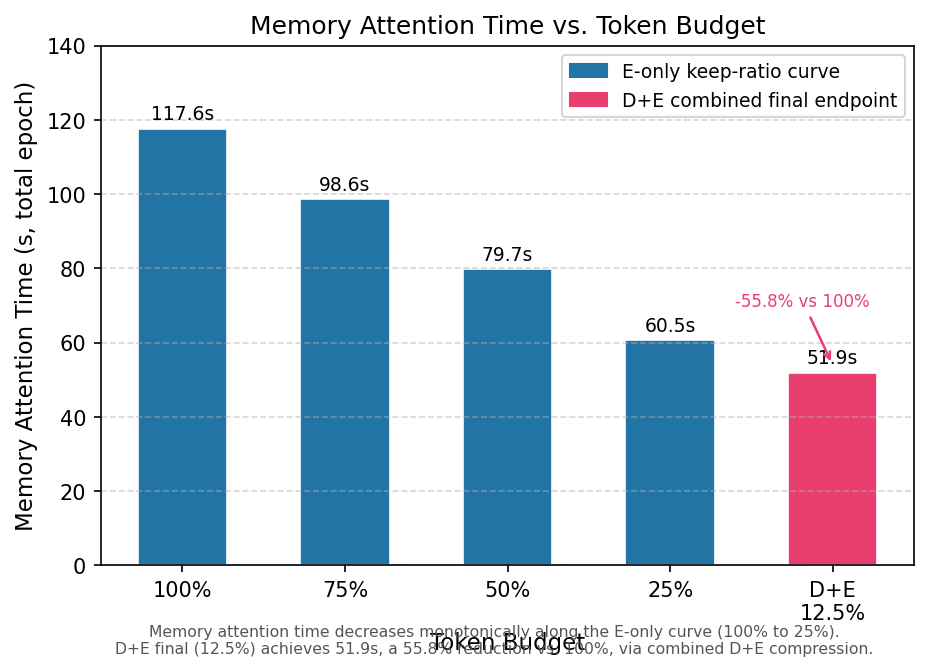
\includegraphics[width=\linewidth]{figures/fig_token_budget_attention_time.png}
\caption{Token预算与注意力时间}
\end{subfigure}
\hfill
\begin{subfigure}{0.48\linewidth}
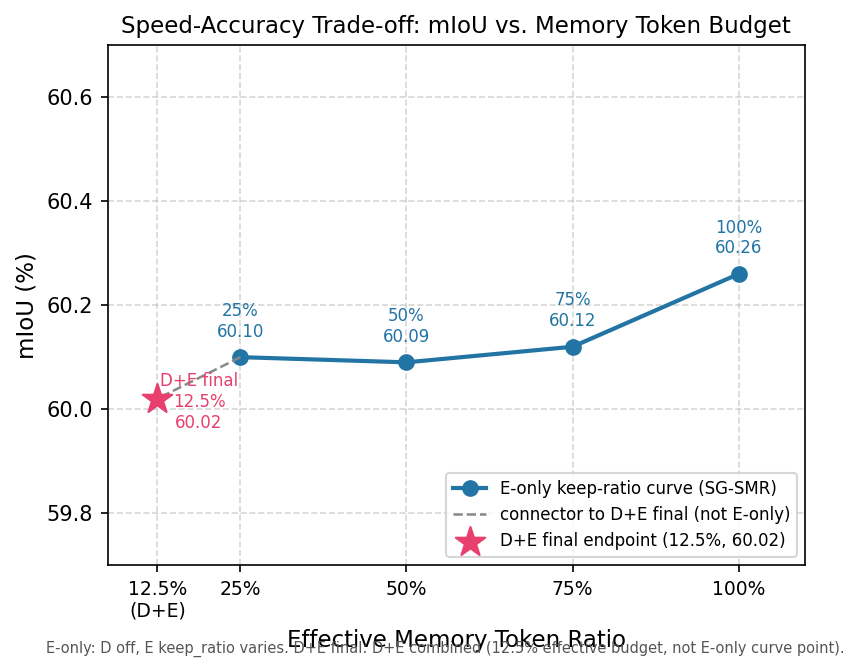
\includegraphics[width=\linewidth]{figures/fig_speed_accuracy_tradeoff_miou.png}
\caption{速度-精度权衡曲线}
\end{subfigure}
\caption{记忆优化的效率分析曲线。(a) 不同Token预算下的注意力计算时间；(b) 压缩率与mIoU的权衡关系。}
\label{fig:efficiency_curves}
\end{figure}
